\documentclass[11pt,aspectratio=43,usenames,dvipsnames]{beamer}
\usepackage[utf8]{inputenc}
\usepackage{amsmath, amsfonts, amssymb, amsthm}
\usepackage[T1]{fontenc}
% mint: code chuck and syntax highlighting
%% outputdir should change according to pdf build directory
\usepackage[outputdir=build,cache=false]{minted}
\usepackage{lmodern}
\usepackage{xcolor}
\usepackage{setspace}
\usepackage{booktabs}
\usepackage{multirow}
\usepackage{graphicx}
\usepackage{fontawesome}

\usepackage[mode=tex]{standalone}
\usepackage{tikz}
\usetikzlibrary{decorations}
\usetikzlibrary{decorations.pathreplacing, intersections}
\usepackage{pgfplots}
\usetikzlibrary{calc,positioning}
\usepgfplotslibrary{fillbetween}
\pgfplotsset{compat=newest, scale only axis, width = 10cm}

% ---------------------------------------------------------------------
% Coordinate extraction
% #1: node name
% #2: output macro name: x coordinate
% #3: output macro name: y coordinate
\newcommand{\Getxycoords}[3]{%
    \pgfplotsextra{%
        % using `\pgfplotspointgetcoordinates' stores the (axis)
        % coordinates in `data point' which then can be called by
        % `\pgfkeysvalueof' or `\pgfkeysgetvalue'
        \pgfplotspointgetcoordinates{(#1)}%
        % `\global' (a TeX macro and not a TikZ/PGFPlots one) allows to
        % store the values globally
         \global\pgfkeysgetvalue{/data point/x}{#2}%
         \global\pgfkeysgetvalue{/data point/y}{#3}%
     }%
}
% ---------------------------------------------------------------------

\usepackage{ulem}
\usepackage{hyperref}
\usepackage{booktabs}
\usepackage{babel}
\usepackage{makecell}
\usepackage[para,online,flushleft]{threeparttable}
\usepackage{pdfpages}
\usepackage{tcolorbox}
\usepackage{bm}
\usepackage{appendixnumberbeamer}
\usepackage{natbib}
\usepackage{caption}
\captionsetup[figure]{labelformat=empty}% redefines the caption setup of the figures environment in the beamer class.
\usetheme[compress]{Boadilla}
\usecolortheme{default}
\useoutertheme{miniframes}
\usefonttheme[onlymath]{serif}

\newcommand{\jump}[2]{\hyperlink{#1}{\beamerbutton{#2}}}
\newcommand{\extjump}[2]{\href{#1}{\beamerbutton{#2}}}
\newcommand{\orange}[1]{\textcolor{orange}{#1}}
\newcommand{\red}[1]{\textcolor{red}{#1}}
\newcommand{\blue}[1]{\textcolor{blue}{#1}}
\newcommand{\green}[1]{\textcolor{OliveGreen}{#1}}

\renewcommand{\square}{\scalebox{0.7}{$\blacksquare$ \hspace{0.5em}}}
\setbeamertemplate{itemize item}{\raisebox{0.1em}{\scalebox{0.7}{$\blacksquare$}}}
\setbeamertemplate{itemize subitem}[circle]
\setbeamertemplate{itemize subsubitem}{--}
\setbeamercolor{itemize item}{fg=black}
\setbeamercolor{itemize subitem}{fg=black}
\setbeamercolor{itemize subsubitem}{fg=black}
\setbeamercolor{item projected}{bg=darkgray,fg=white}
\definecolor{blue}{rgb}{0.2, 0.2, 0.7}
\setbeamercolor{alerted text}{fg=blue}
\setbeamertemplate{enumerate items}[circle]


\setbeamertemplate{headline}{}

%==========================================
\let\olditemize=\itemize
\let\endolditemize=\enditemize
\renewenvironment{itemize}{\olditemize \itemsep1em}{\endolditemize}
\let\oldenumerate=\enumerate
\let\endoldenumerate=\endenumerate
\renewenvironment{enumerate}{\oldenumerate \itemsep1em}{ \endoldenumerate}

\DeclareMathOperator*{\argmax}{\arg\!\max}
\DeclareMathOperator*{\E}{\mathbb{E}}
\DeclareMathOperator*{\var}{\rm Var}
\DeclareMathOperator*{\cov}{\rm Cov}

\theoremstyle{definition}
\newtheorem{assume}{Assumption}
\newtheorem{lem}{Lemma}
\newtheorem{proposition}{Proposition}
\newtheorem{thm}{Theorem}
\newtheorem{corol}{Corollary}

\AtBeginSection[]{
  \begin{frame}[noframenumbering]
  \vfill
  \centering
  \begin{beamercolorbox}[sep=8pt,center,shadow=true,rounded=true]{title}
    \usebeamerfont{title}\insertsection\par%
  \end{beamercolorbox}
  \vfill
  \end{frame}
}

\begin{document}
    \title[Unit 14]{Unit 14 \\ Unemployment and Fiscal Policy}
    \author[Hui-Jun Chen]{Hui-Jun Chen}
    \institute[OSU]{The Ohio State University}
    \date{\today}
    \setbeamertemplate{navigation symbols}{}
    \setstretch{1.2}

%-------------------------------------------------------
{
%	\usebackgroundtemplate{\includegraphics[width=1\paperwidth]{../EveningSky_cropped_edit43_bright.jpg}}
    \begin{frame}
% \vspace{3em}
        \centering
%		{\footnotesize 	ECON 4002 Intermediate Macroeconomic Theory}
        \maketitle
% \vspace{-1.5em}
% \centering
% \includegraphics[width=0.55\linewidth]{Pictures/houses.jpeg}


    \end{frame}
}

% -------------------------------------------
\setbeamertemplate{headline}
{
\setbeamercolor{section in head/foot}{fg=black, bg=white}
\vskip1em \tiny \insertsectionnavigationhorizontal{1\paperwidth}{\hspace{0.50\paperwidth}}{}
}
%------------------------------------------

\section[Intro]{Introduction}
\label{sec:Introduction}

\begin{frame}{Introduction \extjump{https://www.core-econ.org/the-economy/book/text/14.html}{Textbook}}
\label{slide:Introduction}

\begin{itemize}
    \item The volatile nature of GDP comes from consumption and investment
    \item The agg. behavior of HH and firms \alert{may} \textbf{destabilize} the economy
    \item Is a \alert{stable economy} good/desirable?
    \begin{itemize}
        \item Stabilization $ \approx $ \underline{control}, recall when \alert{firm} can affect prices
        \item What is the possible narrative to justify \alert{gov} control the price?
    \end{itemize}
    \item If you agree that \alert{stable economy} is desirable, then
    \begin{itemize}
        \item How can the government stabilize the economy?
        \item Why might government policies be ineffective?
        \item How can we model the link between output and unemployment?
    \end{itemize}

\end{itemize}


\end{frame}

\begin{frame}{Introduction (Cont')}
\label{slide:Introduction__Cont__}
    \begin{figure}
        \centering
        
\includegraphics[width=0.8\textwidth]{./figures/1.pdf}
        \caption{Gov spending $ \uparrow  $ in recession $ \Rightarrow  $ already trying to stabilize!}
    \end{figure}
\end{frame}

\section[AD]{The Aggregate Demand function and the Multiplier model}
\label{sec:The_Aggregate_Demand_function_and_the_Multiplier_model}

\begin{frame}{Aggregate Consumption Function}
\label{slide:Aggregate_Consumption_Function}

    \begin{columns}
        \begin{column}{0.3\textwidth}
            Two components of agg. $ C $:
            \begin{enumerate}
                \item \alert{Autonomous consumption}: the fixed amount one will spend, independent of income
                \item Consumption dependent on \alert{income}
            \end{enumerate}
        \end{column}
        \begin{column}{0.7\textwidth}
            \begin{figure}
                \centering
                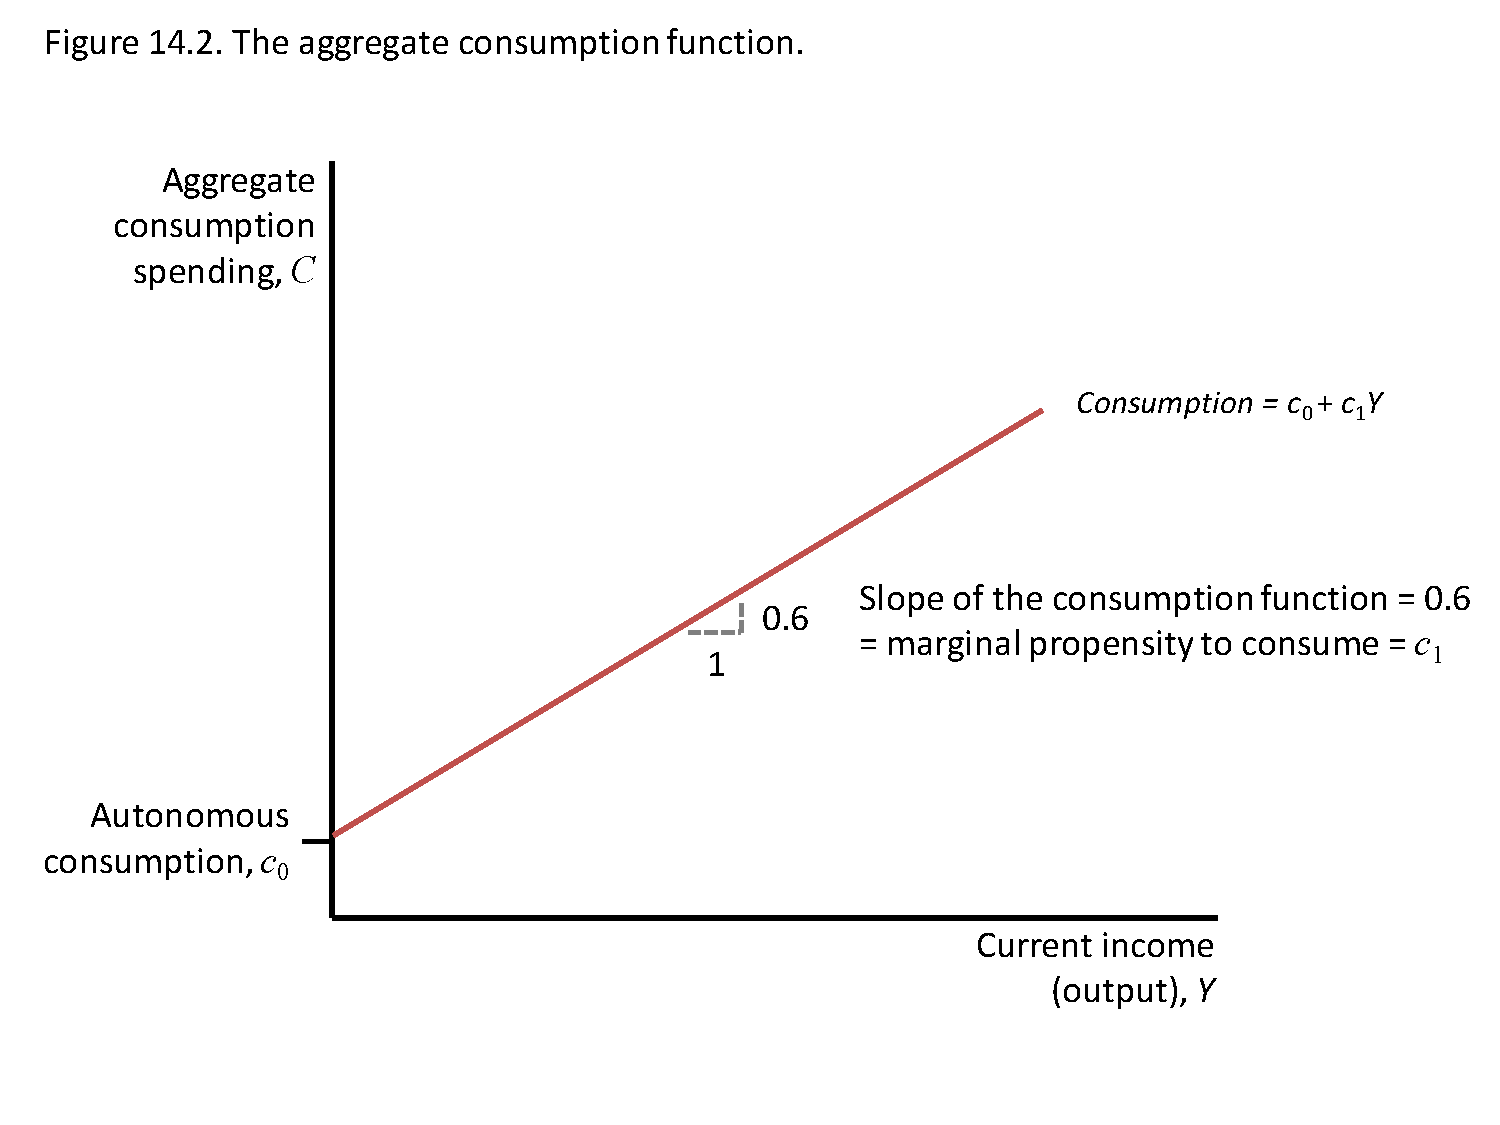
\includegraphics[width=\textwidth]{./figures/2.pdf}
            \end{figure}

        \end{column}
    \end{columns}

\end{frame}

\begin{frame}{Marginal Propensity to Consume (MPC)}
\label{slide:Marginal_Propensity_to_Consume__MPC_}
    Marginal propensity to consume varies across people:
    \begin{itemize}
        \item \textbf{Usually} poor HH has \alert{high} MPC yet rich HH has \alert{low} MPC
        \item Recall $ MPC = \Delta C / \Delta Y$, poor HH's $ C $ reacts much to flow income
        \item Should support poor HH with transfer/tax rebate?

    \end{itemize}
        \vspace{1em}
            \begin{quote}
                Wealthy hand-to-mouth households -who hold \alert{little or no liquid wealth} despite owning sizable quantities of \alert{illiquid assets}- can help accounting for the \alert{large estimated propensities to consume} out of (small) tax rebates. \hfill-- \cite{Kaplan_Violante_2014_Econometrica}
            \end{quote}

\end{frame}

\begin{frame}{Goods Market Equilibrium}
\label{slide:Goods_Market_Equilibrium}
    \begin{columns}
        \begin{column}{0.3\textwidth}
            \begin{itemize}
                \item Aggregate demand (AD) $ = C + I$
                \begin{itemize}
                    \item investment is assumed to be independent of output ($ Y $)
                \end{itemize}
                \item the slope of AD line is below 45° because $MPC<1$
            \end{itemize}

        \end{column}
        \begin{column}{0.7\textwidth}
            \begin{figure}
                \centering
                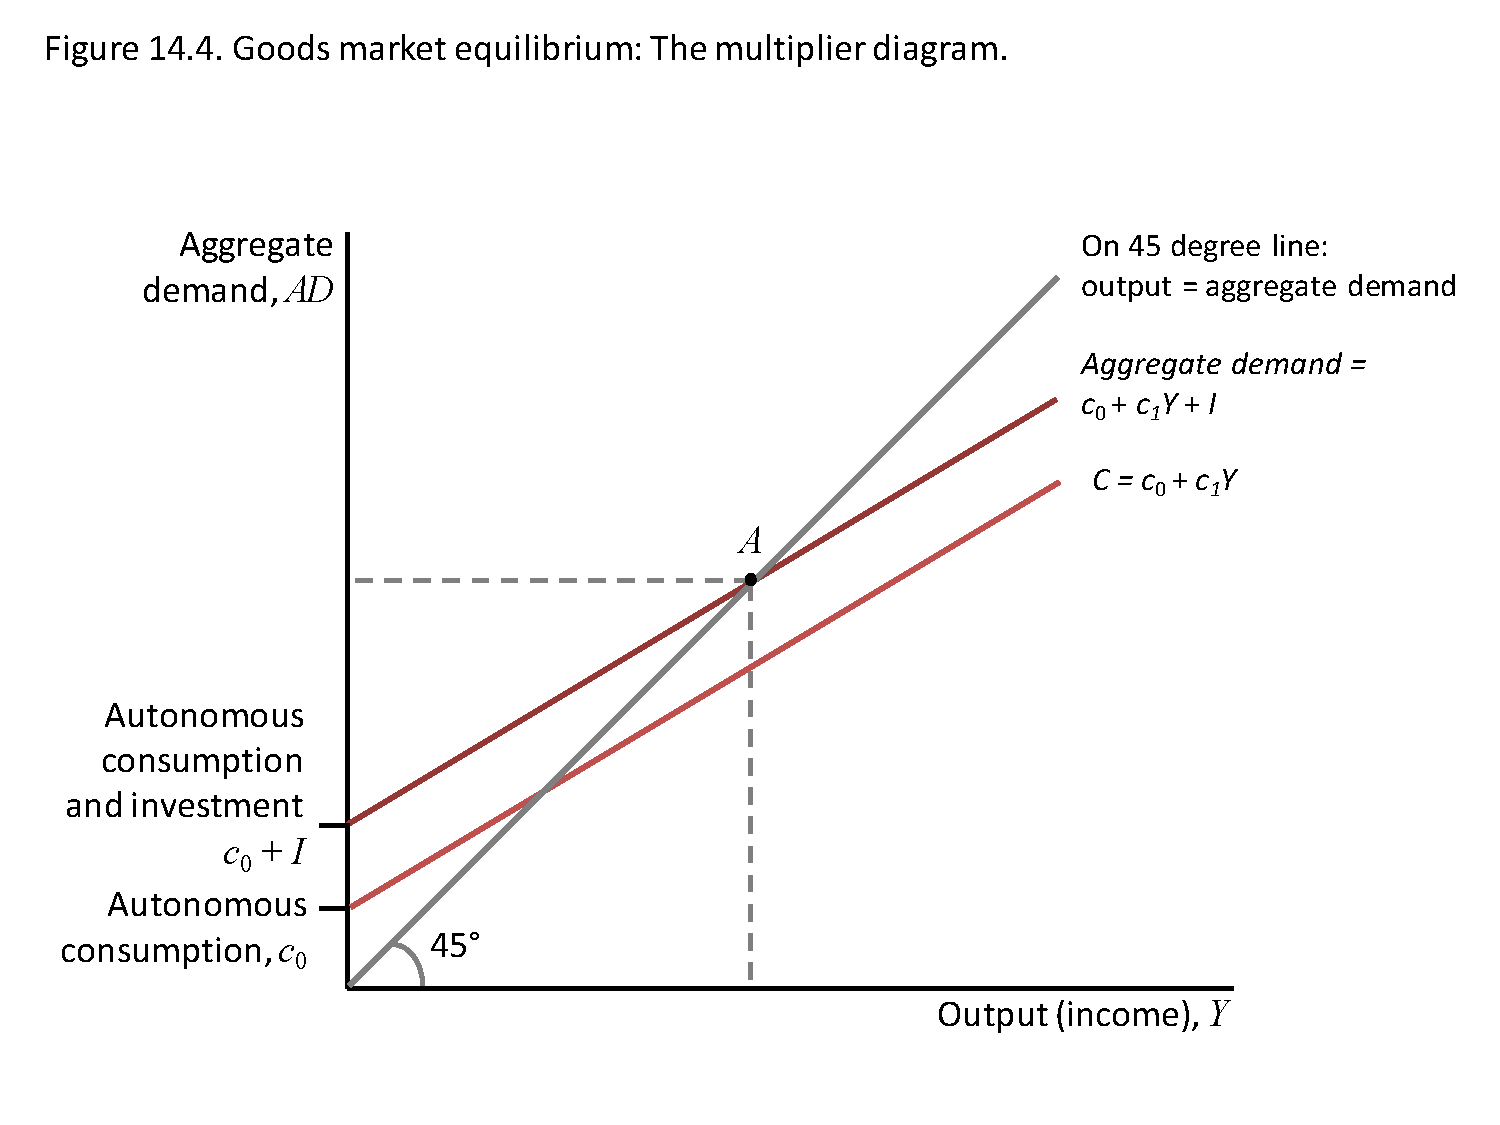
\includegraphics[width=\textwidth]{./figures/4.pdf}
                \caption{Goods Market Eq: $ Y = AD $}
            \end{figure}

        \end{column}
    \end{columns}

\end{frame}

\begin{frame}{The Multiplier Process}
\label{slide:The_Multiplier_Process}
    \begin{columns}
        \begin{column}{0.5\textwidth}
            \only<1>{
            \begin{itemize}
                \item Fall in investment
                \item → fall in aggregate demand
                \item → lower output and income
                \item → further fall in demand and income
                \item → new equilibrium (Z)
                \item Why multiplier $ = \frac{1}{1 - MPC} $?
            \end{itemize}
            }
            \only<2>{
            \begin{itemize}
                \item $ MPC = \frac{\Delta C}{\Delta Y} $
                \item Imagine an economy with only $ 2 $ person
                \item The initial increase in spending is $ \$x $, from A to B
                \item B will spend $ \$x \times MPC $ back to A
            \end{itemize}
            }
            \only<3>{
            \begin{itemize}
                \item This process continues, and the total increase in GDP is
                        %
                        \begin{equation*}
                            \begin{split}
                                    & \$x \cdot 1 + \$x \cdot MPC
                                \\
                                    & \quad + \$x \cdot MPC^{2} + \cdots
                                \\
                                    & = \$x \cdot ( 1 + MPC
                                \\
                                    & \quad + MPC^{2} + \cdots )
                                \\
                                    & = \$x \cdot \underbrace{\frac{1}{1 - MPC}}_{\text{multiplier}}
                                \\
                            \end{split}
                        \end{equation*}
                        %
            \end{itemize}
            }

        \end{column}
        \begin{column}{0.6\textwidth}
            \only<1>{
            \begin{figure}
                \centering
                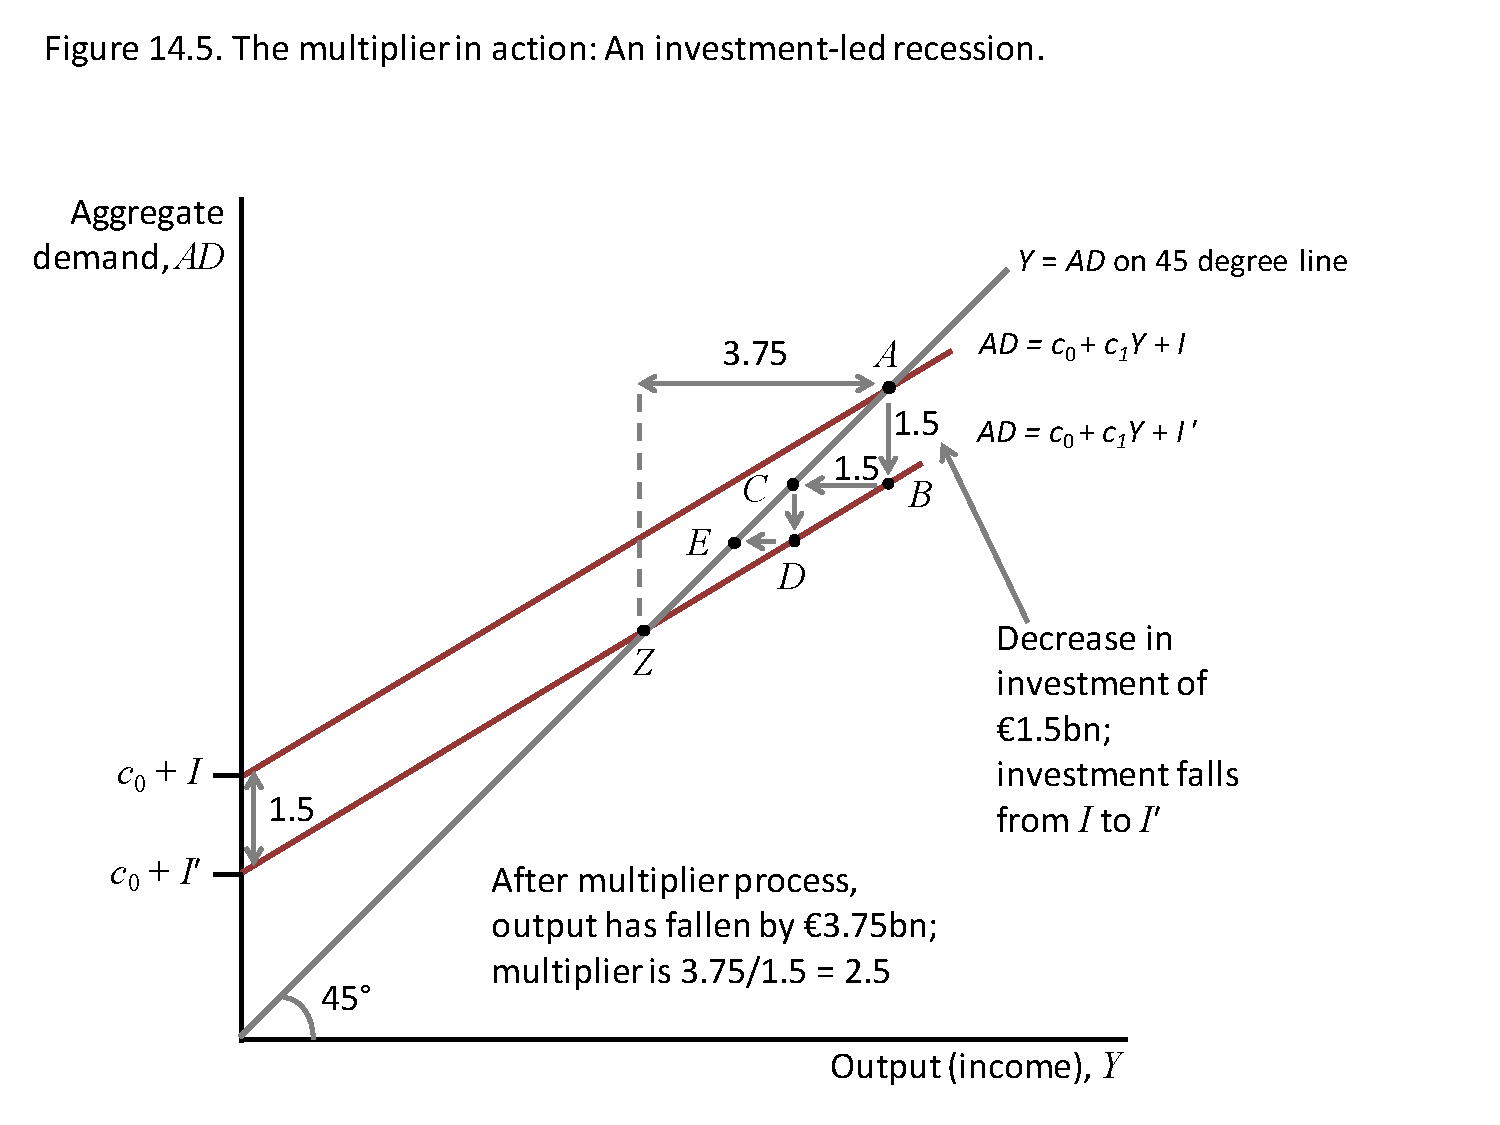
\includegraphics[trim = {0.5cm 0.5cm 1.5cm 0.5cm}, clip, width=\textwidth]{./figures/5.pdf}
                \caption{Multiplier $ = \frac{1}{1 - MPC} $}
            \end{figure}
            }
            \only<2-3>{
            \begin{tikzpicture}
                \pgfmathsetmacro{\x}{5}
                \pgfmathsetmacro{\y}{1}
                % \draw[very thin,color=gray, step=1] (0,0) grid (\x, \y); % gray grid
                \draw[very thick, blue, ->] (1, 0.3) to[bend left=50] node[above]{\$x} (5, 0.3);
                \draw[very thick, blue, <-] (1, 0) to[bend right=50] node[below]{\$x $\times$ MPC} (5, 0);
                \draw[very thick, orange, ->] (1, 0.2) to[bend left=30] node[below]{\$x $\times$ MPC$^2$} (5, 0.2);
                \draw[very thick, orange, <-] (1, 0.1) to[bend right=30] node[above]{\$x $\times$ MPC$^3$} (5, 0.1);
                \fill (1, 0.15) circle (2pt) node[above, rotate=90]{A};
                \fill (5, 0.15) circle (2pt) node[above, rotate=270]{B};
            \end{tikzpicture}
            }

        \end{column}
    \end{columns}

\end{frame}

\begin{frame}{The Multiplier Effect}
\label{slide:The_Multiplier_Effect}
    \begin{itemize}
        \item $ \Delta Y $ can be greater than the initial change in aggregate demand.
        \item The multiplier represents the relative \textit{magnitude} of this change.
        \begin{itemize}
            \item multiplier $= 1$: the increase in GDP $ = $ the initial increase in spending
            \item multiplier $> (<) 1$: the total increase in GDP $> (<)$ the initial increase in spending
        \end{itemize}
        \item Credit constraints and consumption smoothing is reflected in the slope of the AD curve and the size of the multiplier.
        \item Consumption decisions can also shift the AD curve.
        \begin{itemize}
            \item e.g. a fall in house prices will be bad news for a household with a mortgage. They may choose to save more (precautionary saving) and hence their autonomous consumption would fall.
        \end{itemize}

    \end{itemize}
\end{frame}

\begin{frame}{Example: The Great Depression}
\label{slide:Example__The_Great_Depression}

    \begin{figure}
        \centering
        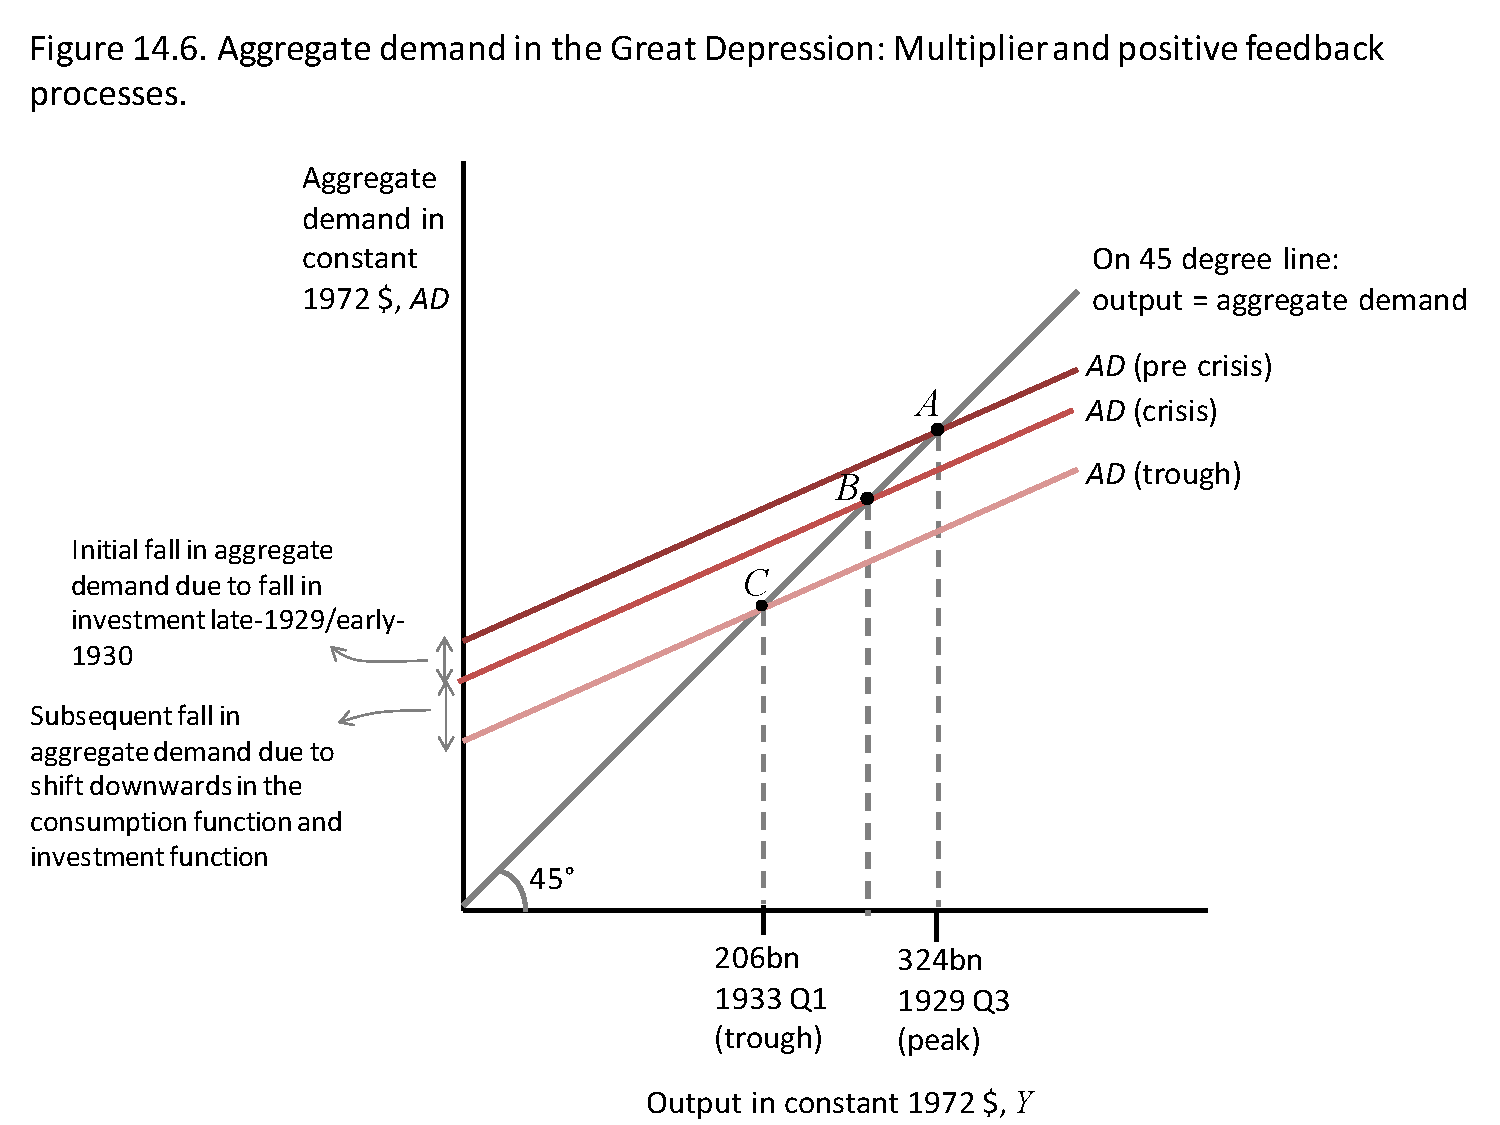
\includegraphics[width=0.9\textwidth]{./figures/7.pdf}
        \caption{}
    \end{figure}
\end{frame}

\section[$C$]{Household Wealth}
\label{sec:Household_Wealth}


\begin{frame}{Household Wealth}
\label{slide:Household_Wealth}
    \begin{figure}
        \centering
        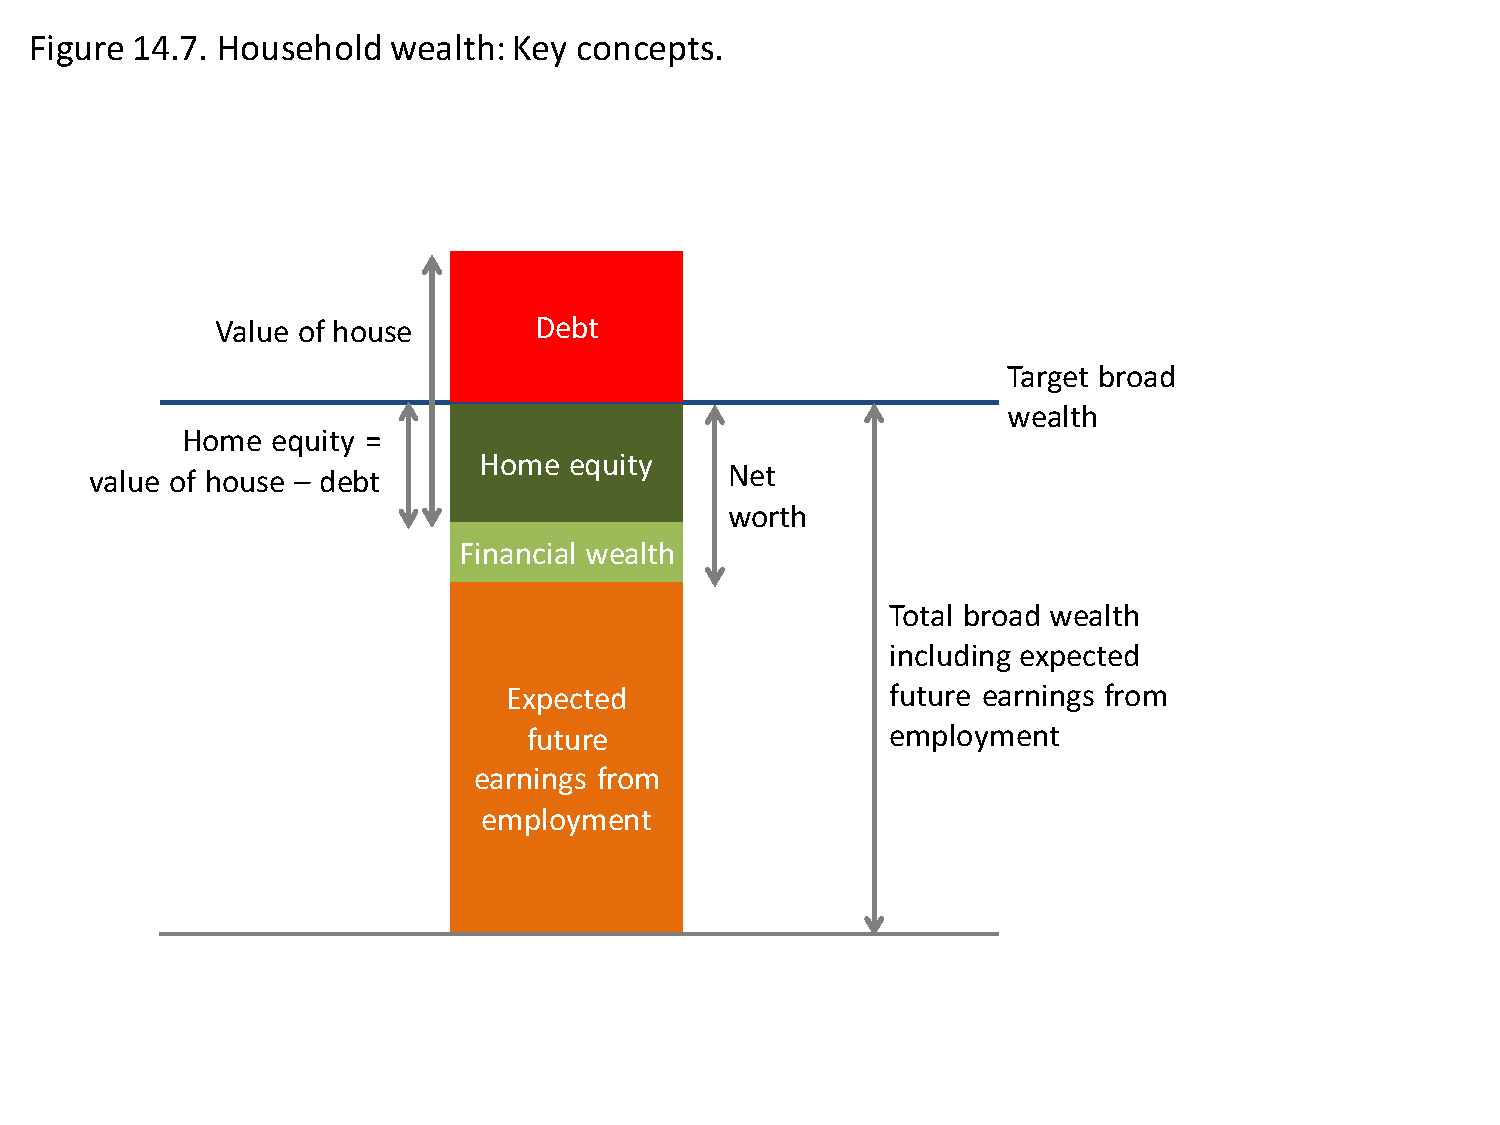
\includegraphics[width=0.8\textwidth]{./figures/8.pdf}
        \caption{Household wealth impacts autonomous consumption}
    \end{figure}

\end{frame}

\begin{frame}{Precautionary Saving}
\label{slide:Precautionary_Saving}
    \begin{columns}
        \begin{column}{0.4\textwidth}
            \begin{itemize}
                \item \textbf{Target wealth}: the level of wealth that a household aims to hold, based on its economic goals (or preferences) and expectations.
                \item \textbf{Precautionary saving}: An increase in saving to restore wealth to its target level.
            \end{itemize}
        \end{column}
        \begin{column}{0.6\textwidth}
            \begin{figure}
                \centering
                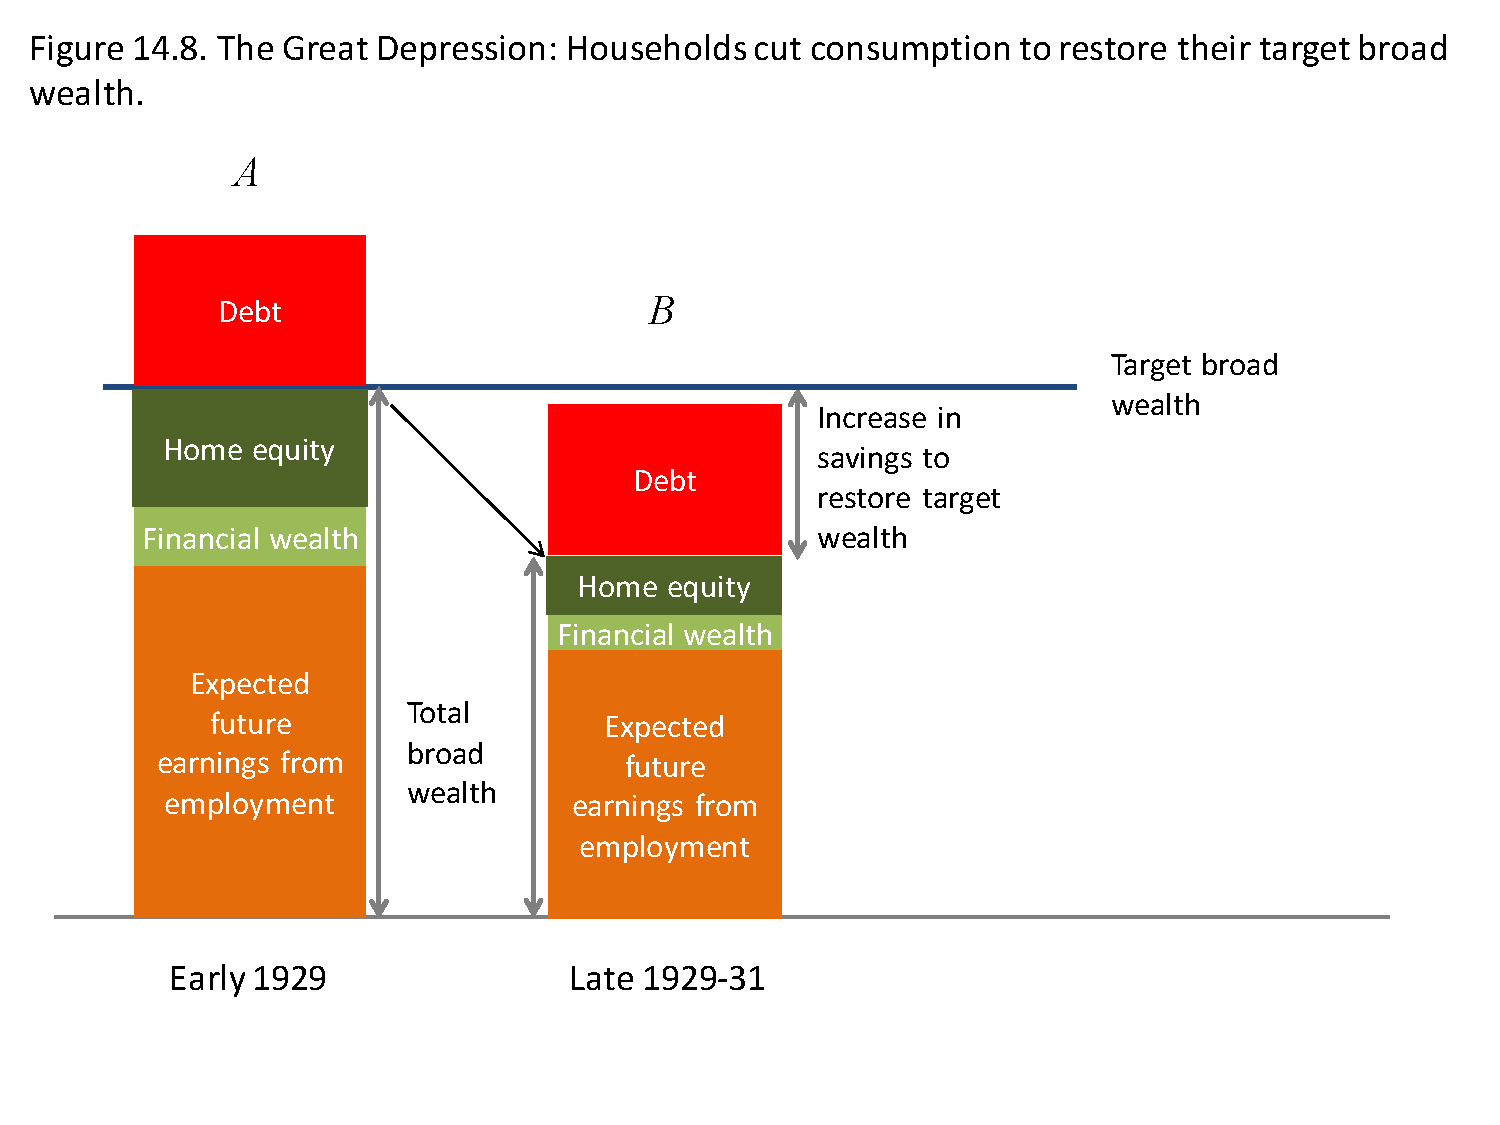
\includegraphics[width=\textwidth]{./figures/9.pdf}
                \caption{Expected earning $ \downarrow  \Rightarrow C \downarrow $ to restore target wealth.}
            \end{figure}

        \end{column}
    \end{columns}

\end{frame}

\begin{frame}{Housing Market}
\label{slide:Housing_Market}
    Changes in house prices affect consumption through two channels:
    \begin{enumerate}
        \item Via change in household wealth (home equity)
        \item Via change in credit constraints: lower house value makes it more difficult to borrow (greater credit constraint)
    \end{enumerate}


\end{frame}

\section[$I$]{Investment}
\label{sec:Investment}


\begin{frame}{Investment Spending}
\label{slide:Investment_Spending}
    Firms’ decision about what to do with its profits depends on
    \begin{itemize}
        \item Owner’s discount rate $ (\rho) $ Consume
        \item Interest rate on assets $(r)$ Save
        \item Net profit rate on investment $ (\pi) $
    \end{itemize}
    Decision rules are
    \begin{itemize}
        \item \alert{Consume} the extra income (dividends) if $ \rho > r \ge \pi $
        \item \alert{Save} the extra income/repay debts if $ r > \rho \ge \pi $
        \item \underline{\alert{Invest} (at home or abroad) if $ \pi > \rho \ge r $}
        \begin{itemize}
            \item If $ r $ is low, then only comparison is $ \pi $ and $ \rho $
            \item \alert{In principle}, lower interest rate will stimulate investment
        \end{itemize}

    \end{itemize}

\end{frame}

\begin{frame}{Supply side effects}
\label{slide:Supply_side_effects}
    \begin{columns}
        \begin{column}{0.3\textwidth}
            \begin{itemize}
                \item<only@1> \alert{In practice}, $ I $ is not sensitive to interest rate
                \item<only@1> \textbf{Aggregate investment} shows how investment spending in the economy as a whole depends on other variables
                \item<only@2> For developing countries, improvement in \textbf{business environment} (such as fall in the \textbf{risk of expropriation} by the government) is more important
            \end{itemize}

        \end{column}
        \begin{column}{0.7\textwidth}
            \begin{figure}
                \centering
                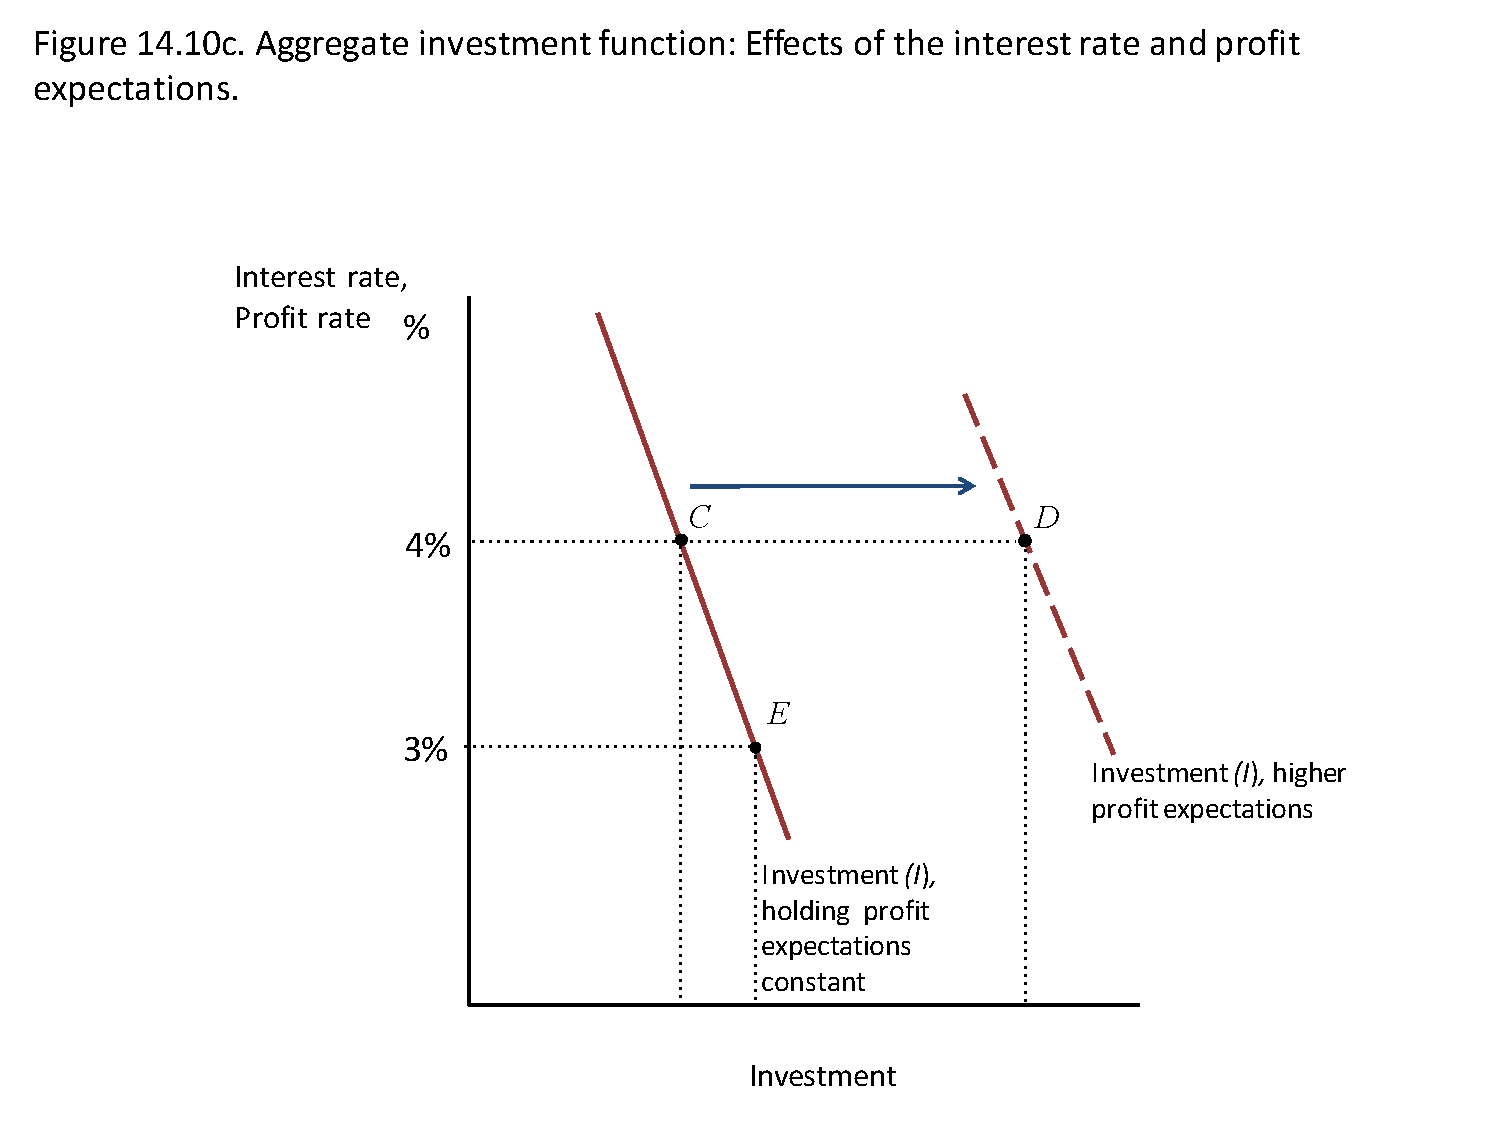
\includegraphics[width=\textwidth]{./figures/13.pdf}
                \caption{}
            \end{figure}

        \end{column}
    \end{columns}

\end{frame}

\section[\faBuildingO]{The role of government}
\label{sec:The_role_of_government}

\begin{frame}{GDP Expenditure Approach and Government Intervention}
\label{slide:GDP_Expenditure_Approach}
    %
    \begin{equation}
        AD = C + I + G + EX - IM
    \end{equation}
    %
    \begin{itemize}
        \item $ C $: $ MPC $ and disposable income $(1-\tau) Y$
        \item $ I $: interest rate $ r $ and after-tax profit $ (1 - \tau) \pi $
        \item $ G $: exogenous, shift AD curve in parallel
        \item $ EX $: exogenous
        \item $ IM $: depends on domestic income $ Y $ with marginal propensity to import $ m $
    \end{itemize}
    %
    \begin{equation*}
        AD = c_{0} + MPC \times (1 - \tau) Y + I + G + EX - m Y
    \end{equation*}
    %

\end{frame}

\begin{frame}{Stabilizing the Economy}
\label{slide:Stabilizing_the_Economy}
    %
    \begin{equation*}
        AD = c_{0} + MPC \times (1 - \tau) Y + I + G + EX - m Y
    \end{equation*}
    %
    \begin{itemize}
        \item Government spending is large and exogenous
        \item Higher tax rate lowers the multiplier
        \item Unemployment insurance helps households smooth consumption
        \begin{itemize}
            \item market failure $ \because $ correlated risk, hidden actions, hidden attributes
        \end{itemize}
        \item Deliberate intervention via fiscal policy
    \end{itemize}
    The \underline{unemployment benefit scheme} and \underline{proportional tax rate} are \alert{automatic stabilizers}: they \alert{automatically offset} an expansion or contraction of the economy.


\end{frame}

\begin{frame}{What is the multiplier with both MPC and MPI?}
\label{slide:What_is_the_multiplier_with_both_MPC_and_MPI_}
    \begin{columns}
        \begin{column}{0.4\textwidth}
            \begin{itemize}
                \item<only@1> $ MPC $: propensity to consume
                \item<only@1> $ MPI $: propensity to consume \alert{imported goods}
                \item<only@1> $ ? $ is propensity to consume \alert{domestic goods}:
                \item<only@2> For every $\$x$ increase in income, total consumption increase by $ \$x \times MPC $, while consumption for imported goods increase by $ \$x \times MPI $
                \item<only@2> $ \Rightarrow $ consumption for \alert{domestic goods} increase by $\$x \times (MPC - MPI) $ amount.
                \item<only@3> Following the same iterative process, the multiplier of the economy is
                %
                \begin{equation*}
                    \frac{1}{1 - (MPC - MPI)}
                .\end{equation*}
                %
            \end{itemize}
        \end{column}
        \begin{column}{0.6\textwidth}
            \begin{tikzpicture}
                \pgfmathsetmacro{\x}{5}
                \pgfmathsetmacro{\y}{5}
                % \draw[very thin,color=gray, step=1] (0,0) grid (\x, \y); % gray grid
                \draw[very thick, blue, ->] (1, 0.3) to[bend left=50] node[above]{\$x} (5, 0.3);
                \draw[very thick, blue, <-] (1, 0) to[bend right=50] node[below]{\$x $\times$ ?} (5, 0);
                \draw[very thick, orange, ->] (1, 0.2) to[bend left=30] node[below]{\$x $\times$ ?$^2$} (5, 0.2);
                \draw[very thick, orange, <-] (1, 0.1) to[bend right=30] node[above]{\$x $\times$ ?$^3$} (5, 0.1);
                \fill (1, 0.15) circle (2pt) node[above, rotate=90]{A};
                \fill (5, 0.15) circle (2pt) node[above, rotate=270]{B};
                \fill (3.0, 2.85) circle (2pt) node[above]{C};
                \draw[very thick, red, ->] (1, 0.4) to[bend left = 50] node[above, rotate=45] {\$x $\times $ MPI} (3, 2.85);
                \draw[very thick, red, ->] (5, 0.4) to[bend right = 50] node[above, rotate=315] {\$x $\times $ MPI} (3, 2.85);
            \end{tikzpicture}

        \end{column}
    \end{columns}

\end{frame}



\begin{frame}{The paradox of thrift}
\label{slide:The_paradox_of_thrift}
    \begin{itemize}
        \item In a recession, faced with a household budget deficit, a family worried about their falling wealth cuts spending and saves more.
        \item But in the economy as a whole, \alert{spending and earning go together.}
        \item \textbf{The paradox of thrift}: the aggregate attempt to increase savings leads to a fall in aggregate income.
        \item \alert{Fallacy of composition}: what is true for one part of the economy (a single household) is not true of the whole economy.
    \end{itemize}

\end{frame}

\begin{frame}{Fiscal stimulus}
\label{slide:Fiscal_stimulus}
    \begin{columns}
        \begin{column}{0.3\textwidth}
            \begin{itemize}
                \item gov counteract the fall of AD via \alert{fiscal stimulus}:
                \begin{itemize}
                    \item \alert{cut taxes} to encourage the private sector to spend more
                    \item \alert{increase spending (G)}, which directly increases AD
                \end{itemize}

            \end{itemize}

        \end{column}
        \begin{column}{0.7\textwidth}
            \begin{figure}
                \centering
                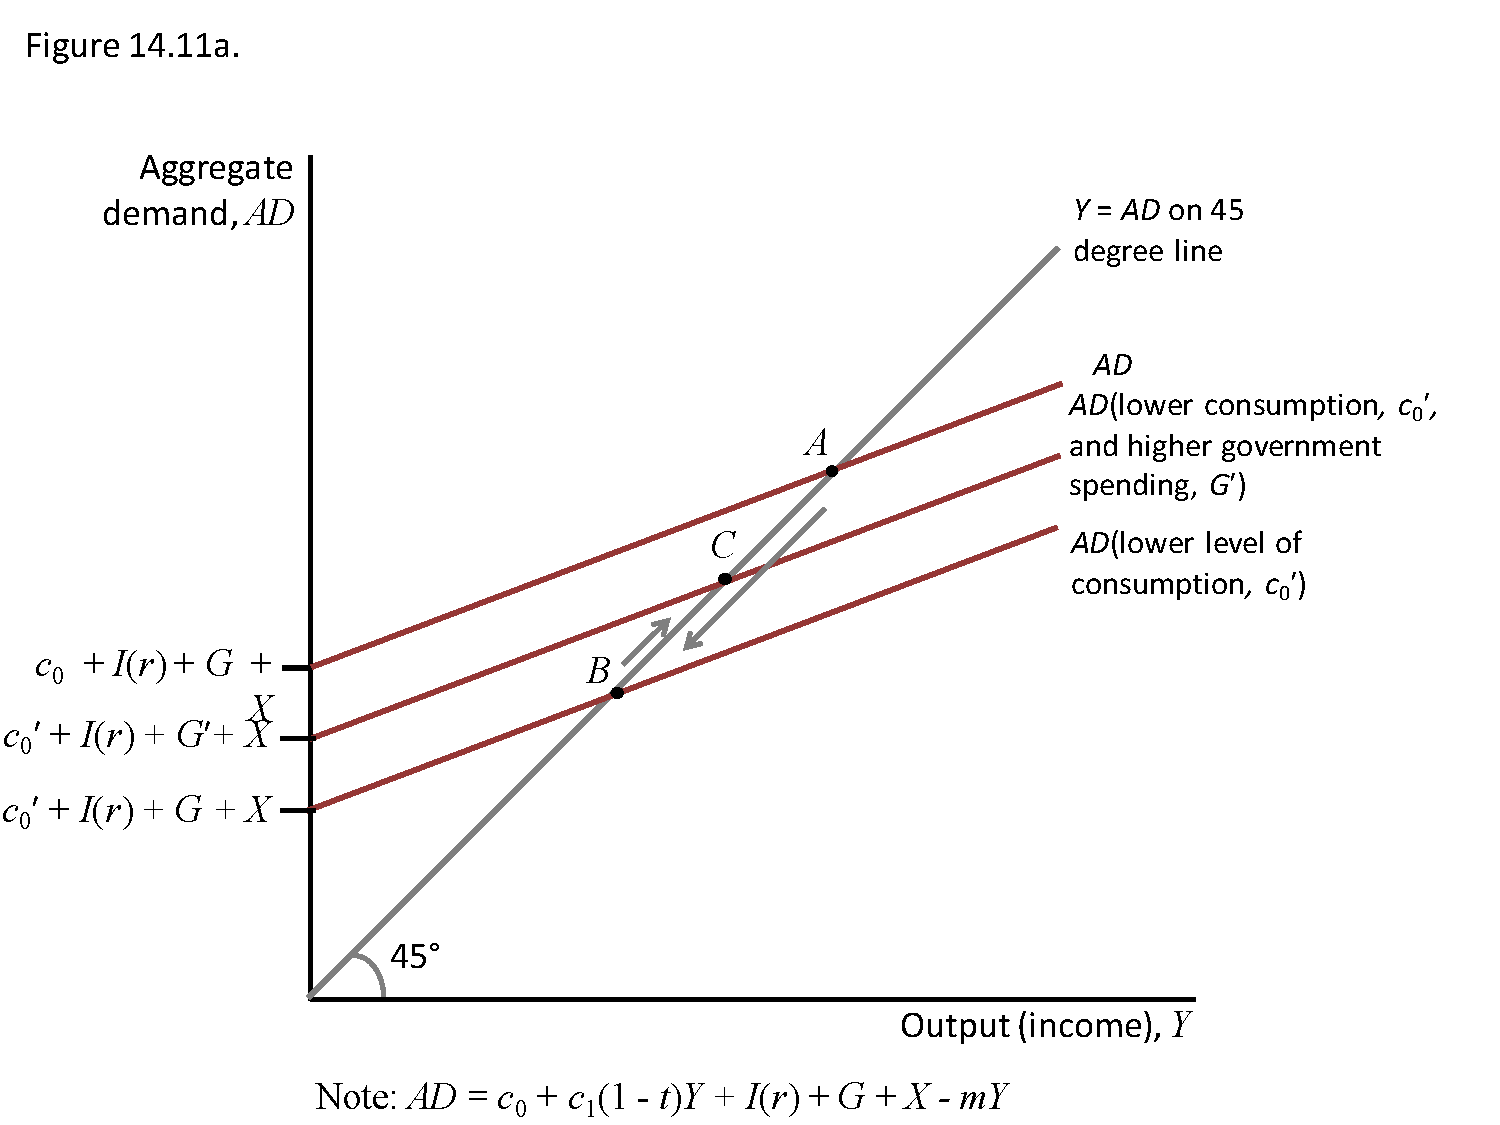
\includegraphics[width=\textwidth]{./figures/14.pdf}
                \caption{$G \uparrow \Rightarrow Y\uparrow \uparrow $ because of multiplier}
            \end{figure}

        \end{column}
    \end{columns}

\end{frame}

\begin{frame}{Financing Fiscal Stimulus}
\label{slide:Financing_Fiscal_Stimulus}
    \begin{center}
        Budget balance $ = T - G $
    \end{center}

    \begin{columns}
        \begin{column}{0.4\textwidth}
            \begin{itemize}
                \item Fiscal stimulus $ \Rightarrow  $ negative budget balance (government \textbf{budget deficit}).
                \item Not reversed after the recession $ \Rightarrow  $ \alert{increase government debt}.
            \end{itemize}
        \end{column}
        \begin{column}{0.6\textwidth}
            \begin{figure}
                \centering
                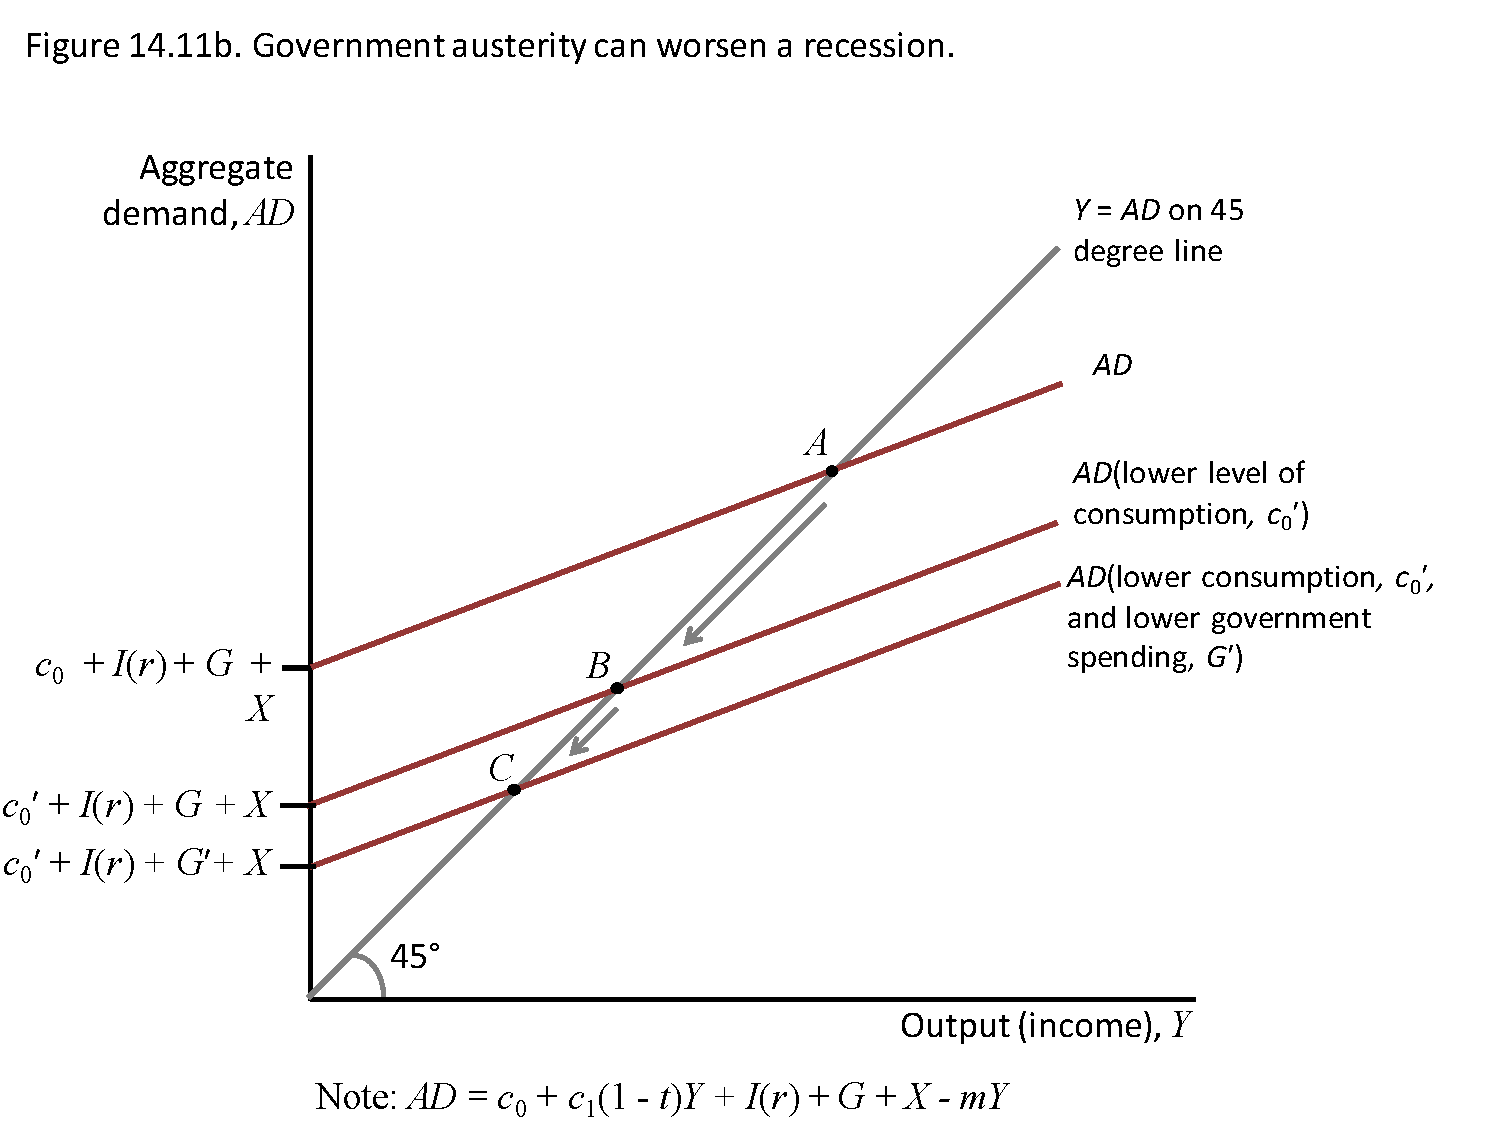
\includegraphics[width=\textwidth]{./figures/15.pdf}
                \caption{}
            \end{figure}

        \end{column}
    \end{columns}
\end{frame}

\begin{frame}{Positive/Negative Feedback Mechanisms}
\label{slide:Positive_Negative_Feedback_Mechanisms}
    \begin{figure}
        \centering
        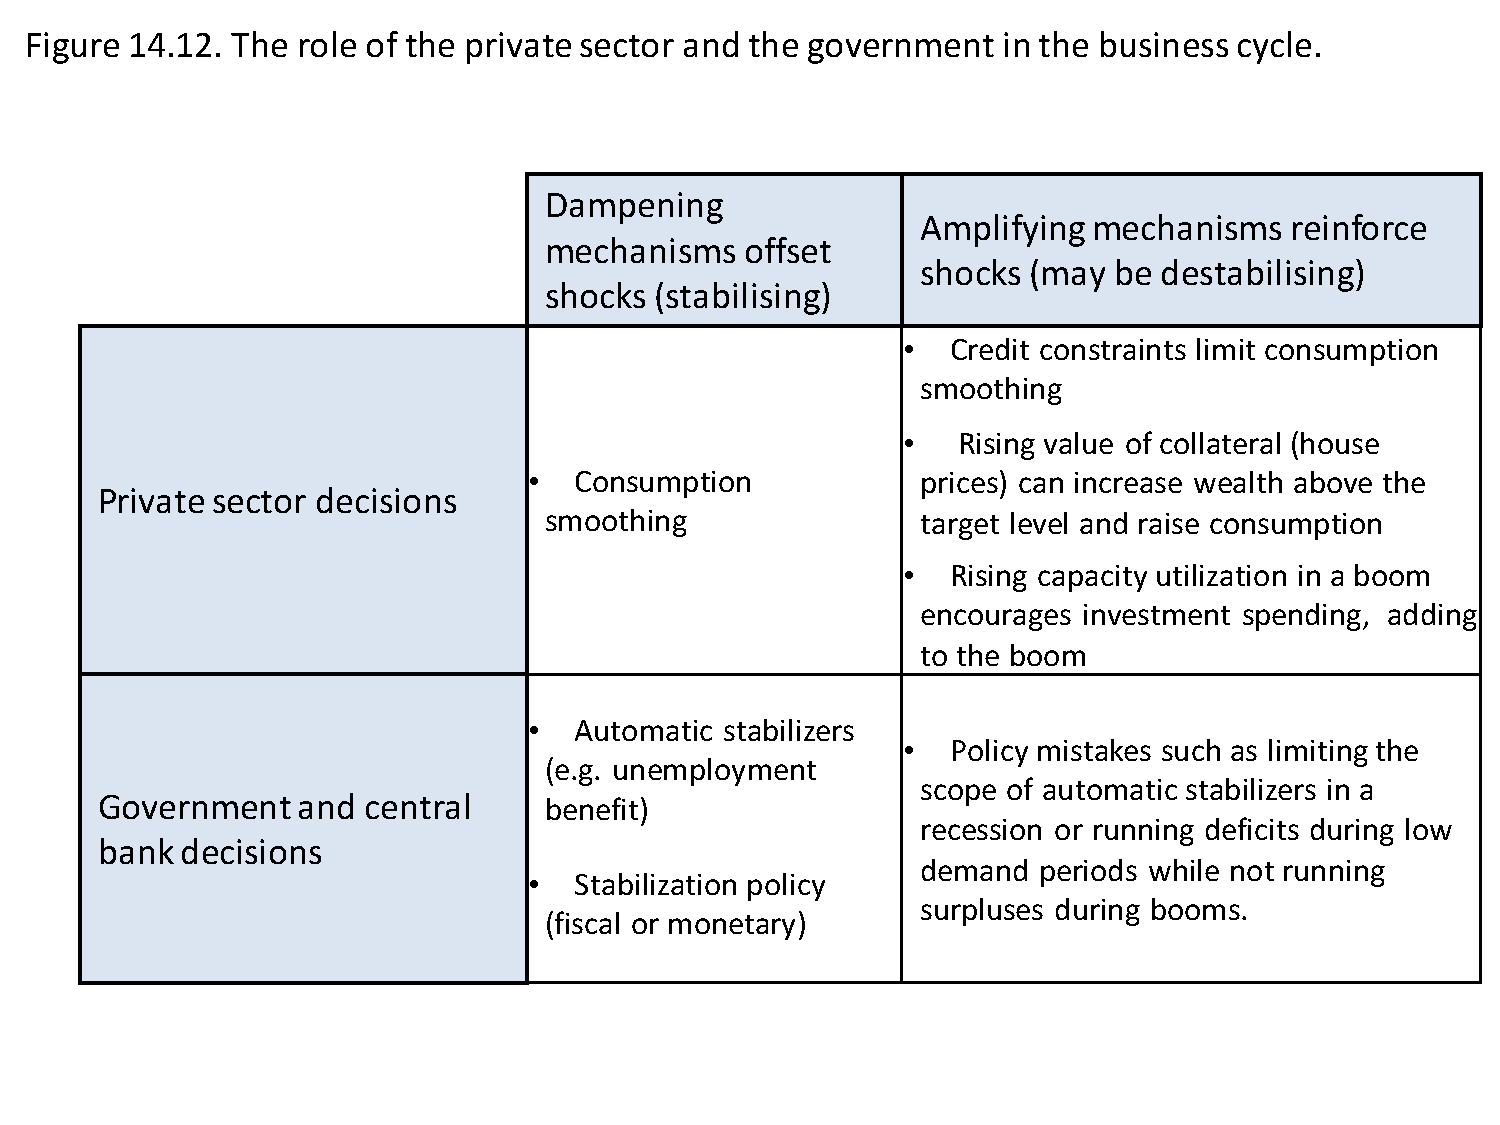
\includegraphics[width=\textwidth]{./figures/16.pdf}
    \end{figure}

\end{frame}

\begin{frame}{Multiplier Model is not telling Whole Story}
\label{slide:Multiplier_Model_is_not_telling_Whole_Story}
    \begin{itemize}
        \item In our model of aggregate demand, the multiplier depended only on the MPC, MPI (IM), and the tax rate.
        \item In reality, it also depends on:
        \begin{itemize}
            \item \textbf{crowd out effect}: if economy is in full capacity utilization, an $ G \uparrow  $ crowd out private spending
            \item \textbf{expectations} of the private sector: the multiplier could be \alert{negative}, recall investment coordination game!
        \end{itemize}
        \item Gov might not be omnipotent:
        \begin{itemize}
            \item \textbf{Sovereign debt crisis}: a situation in which government bonds come to be considered risky (default risk).
            \item \textbf{Debt ceiling}: increase the default risk for US.
        \end{itemize}


    \end{itemize}



\end{frame}

\begin{frame}{Debt-to-GDP ratio}
\label{slide:Debt_to_GDP_ratio}
    \begin{center}
        \textbf{Def}:  level of indebtedness of a gov is measured over the economy size
    \end{center}
    \begin{columns}
        \begin{column}{0.3\textwidth}
            Indebtedness can fall
            \begin{itemize}
                \item if the primary budget balance is positive
                \item if GDP is growing faster than government debt
                \item if inflation is high (real value of debt falls)
            \end{itemize}


        \end{column}
        \begin{column}{0.7\textwidth}
            \begin{figure}
                \centering
                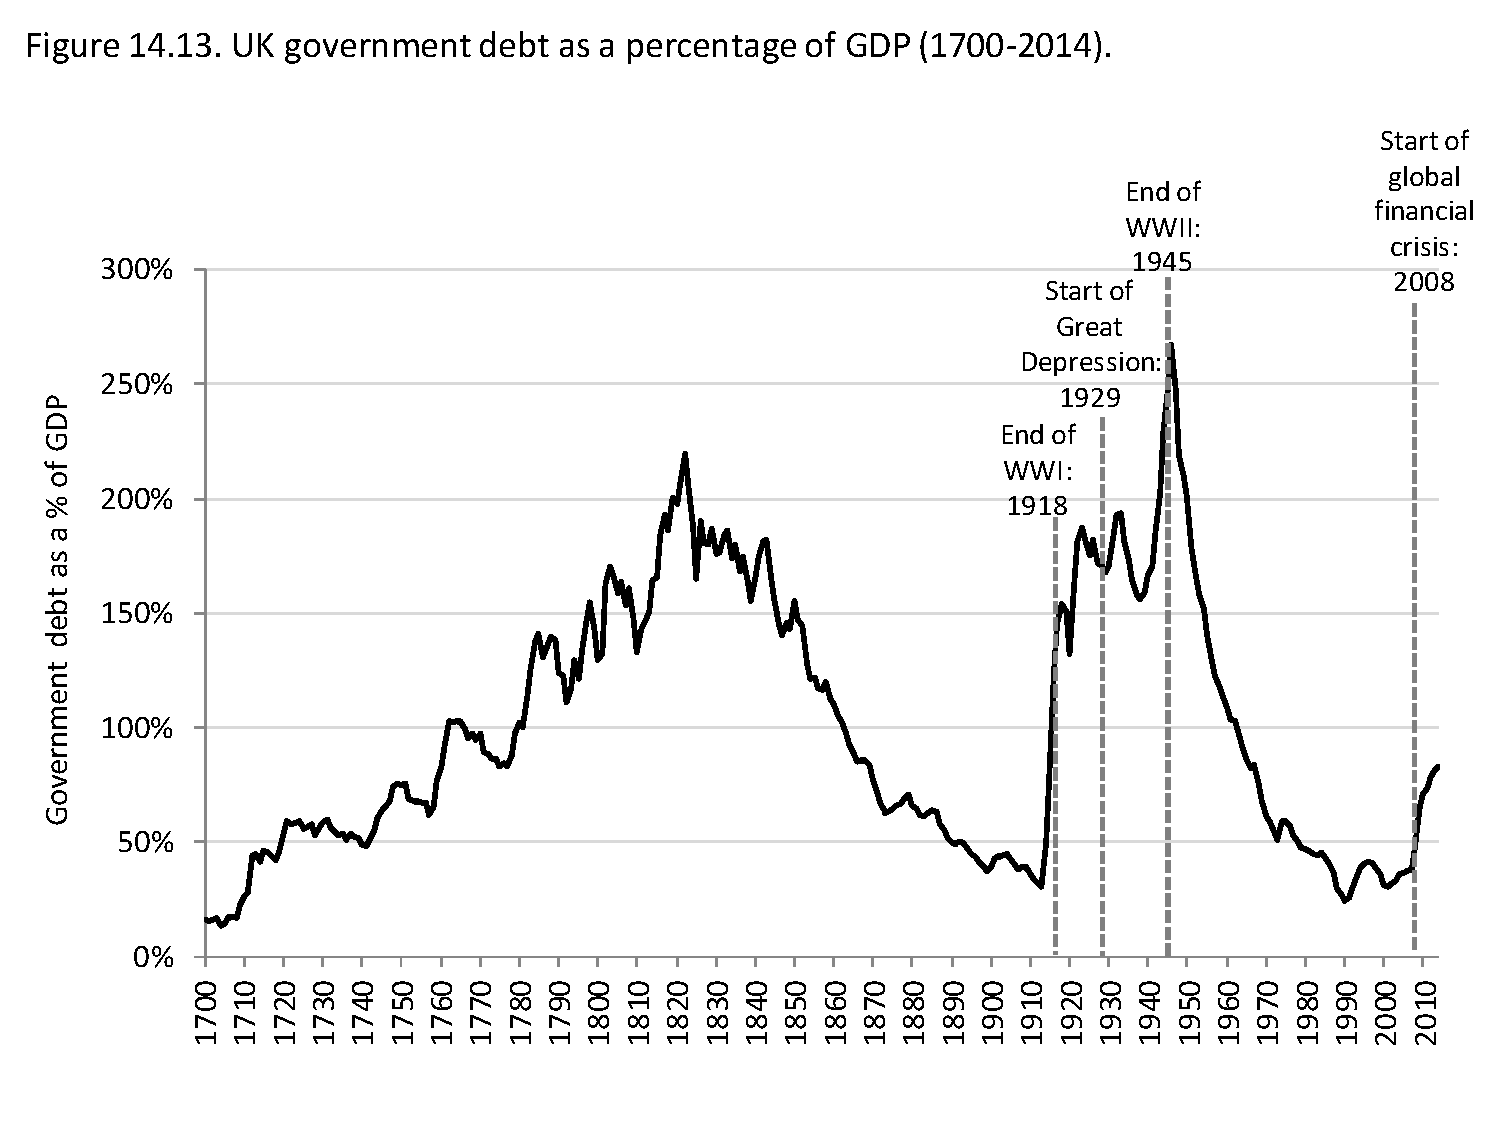
\includegraphics[width=\textwidth]{./figures/17.pdf}
            \end{figure}

        \end{column}
    \end{columns}

\end{frame}

\begin{frame}{Foreign markets and aggregate demand}
\label{slide:Foreign_markets_and_aggregate_demand}
    \begin{itemize}
        \item Fluctuations in the growth rate of important markets abroad influence the domestic economy via demand for exports.
        \item Demand for imports dampens domestic fluctuations.
        \item Foreign trade limits the use of fiscal stimulus if the marginal propensity to import is large.
    \end{itemize}


\end{frame}

\section[AD \& UE]{Aggregate Demand and Unemployment}
\label{sec:Aggregate_Demand_and_Unemployment}

\begin{frame}{Aggregate Demand and Unemployment}
\label{slide:Aggregate_Demand_and_Unemployment}
    \begin{columns}
        \begin{column}{0.4\textwidth}
            \begin{itemize}
                \item \alert{Supply-side}: labour market model
                \begin{itemize}
                    \item \alert{Medium-run model}: wages and prices can change, but capital stock, technology and institutions are fixed
                \end{itemize}
                \item \alert{Demand-side}: multiplier model
                \begin{itemize}
                    \item \alert{Short-run model}: all variables fixed
                \end{itemize}
                \item Also explain \alert{cyclical unemployment}

            \end{itemize}

        \end{column}
        \begin{column}{0.6\textwidth}
            \begin{figure}
                \centering
                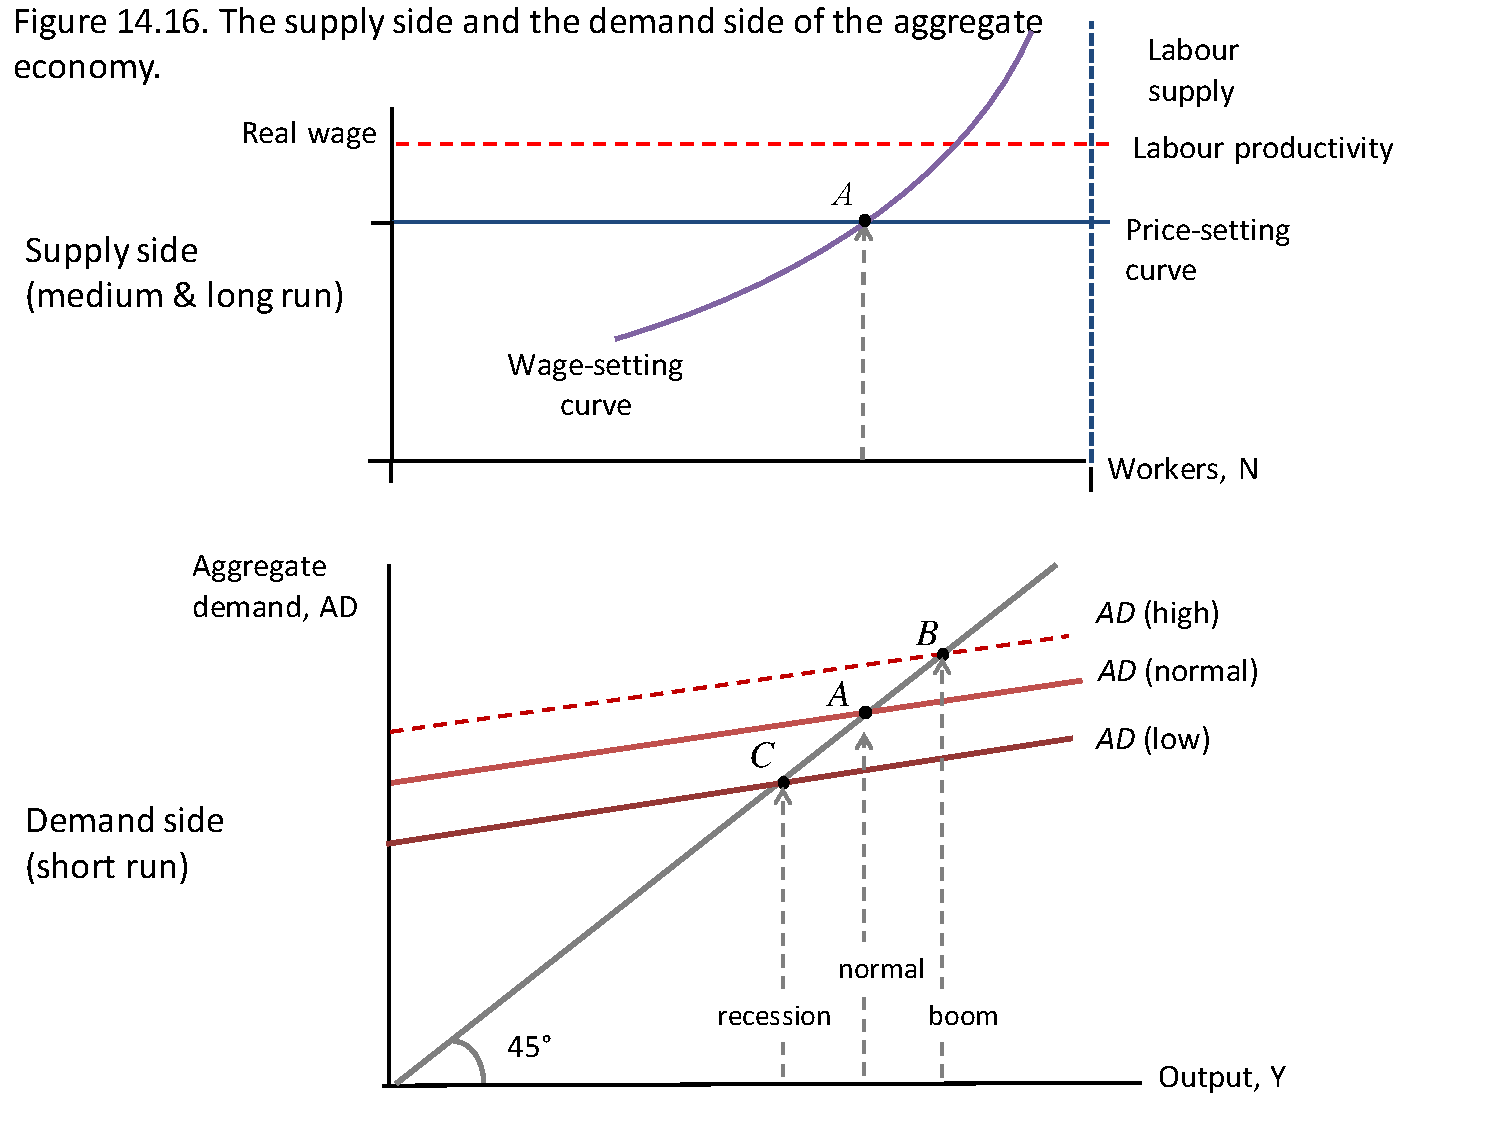
\includegraphics[width=\textwidth]{./figures/19.pdf}
                \caption{Production function connects employment (N) and output (Y)}
            \end{figure}

        \end{column}
    \end{columns}

\end{frame}


\section{Appendix}
\label{sec:Appendix}

\appendix
% -------------------------------------------
\setbeamertemplate{headline}
{
\setbeamercolor{section in head/foot}{fg=black, bg=white}
\vskip1em \tiny \insertsectionnavigationhorizontal{1\paperwidth}{\hspace{0.50\paperwidth}}{}
}
%------------------------------------------
% \begin{frame}\frametitle{}
% \begin{columns}
% \label{Appendix}
% \column{1\linewidth}
% \centering
% {\Large \alert{Appendix}}
% \end{columns}
% \end{frame}
%------------------------------------------
\begin{frame}[allowframebreaks]{References}
\footnotesize
\bibliographystyle{$BIB_STYLE}
\bibliography{$BIBFILE}
\end{frame}

\end{document}
